\documentclass{article}

\usepackage[MeX]{polski}
\usepackage[utf8]{inputenc}
\usepackage{amsmath}
\usepackage{graphicx}
\usepackage{float}
\usepackage{listings}

\usepackage{xcolor}
\usepackage{soul}
\newcommand{\highlight}[2]{\colorbox{#1}{$\displaystyle #2$}}

\lstset
{ 
    language=C++,
    numbers=left,
    basicstyle=\footnotesize,
    stepnumber=1,
    showstringspaces=false,
    tabsize=1,
    breaklines=true,
    breakatwhitespace=false,
}
\setlength\parindent{0pt}

\author{Jakub Tkacz}
\title{Interpolacja}
\date{11.04.2019}

\begin{document}
    \maketitle

    \pagebreak

    \tableofcontents

    \pagebreak

    \section{Wstęp}
    Program realizujący zadania z labolatorium 5 postanowiłem napisać w C++. 

    Do reprezentacji wielomianów stworzyłem własną klasę Poly, która implementowała również podstawowe operacje matematyczne takie jak (dodawanie, mnożenie, dzielenie).
    Dzięki takiemu podejściu kod funkcji liczącej wielomian stał się dużo czytelniejszy.

    Z uwagi na prostotę rysowania wykresów w R, wszystkie dane eksportowałem do plików csv, a następnie za pomocą pakietu ggplot rysowałem wykresy.

    \subsection{Klasa Poly}
    Klasa Poly zawiera dwa pola: listę dwumianów (Term) oraz stopień wielomianu. Metody w niej zawarte to mnożenie wielomiany przez wielomian, dodawanie wielomianów, dzielenie i mnożenie przez stałą.
    \lstset {language=C++}
    \begin{lstlisting}[caption={Klasa Poly}]
class Poly {
private:
    std::list<Term> terms;
    int degree;
public:
    Poly();

    Poly(const std::list<Term> &terms);

    Poly operator*(Poly const &obj);

    Poly operator+(Poly const &obj);

    Poly operator/(double const &d);

    Poly operator*(double const &d);

    double calculate(double x) {
        double ret = 0.0;
        for (auto term: terms)ret += term.calculate(x);
        return ret;
    }

    std::string toString();
};
    \end{lstlisting}
    \subsection{Klasa Term}
    Dodatkową pomocniczą klasą jest Term, reprezentujący dwumian w postaci $a\cdot x^n$
    
    \lstset {language=C++}
    \begin{lstlisting}[caption={Klasa Term}]
class Term {
private:
    double coefficient;
    int exponent;
public:
    Term(double coefficient, int exponent);

    Term();

    Term add(double coefficient);

    double getCoefficient();

    int getExponent();

    double calculate(double x) {
        return coefficient * pow(x, exponent);
    }

    std::string toString();
};
    \end{lstlisting}
    \pagebreak

    \section{Interpolacja Lagrange'a}
    \subsection{Wstęp}
    \subsubsection{Wzór na interpolację}
    \begin{displaymath}
        W(x)=\sum^N_{i=0}y_iL_i(x)
    \end{displaymath}
    \begin{displaymath}
            L_i(x)=\prod^{N}_{k=0, k\neq i}\frac{x-x_k}{x_i-x_k}
    \end{displaymath}
    \subsection{Wykonanie}
    Kod funkcji wykonującej interpolację Lagrange'a jest dosłowną realizacją matematycznych wzorów w kodzie programu.
    \subsubsection{Kod}
    \lstset {language=C++}
    \begin{lstlisting}[caption={Interpolacja metodą Lagrange'a}]
Poly lagrangeInterpolation(std::vector<Node> nodes) {
    Poly L[nodes.size()];
    Poly W({Term(0, 0)});
    for (int i = 0; i < nodes.size(); i++) {
        Poly num({Term(1, 0)});
        double denom = 1.0;
        for (int k = 0; k < nodes.size(); k++) {
            if (k != i) {
                Poly b({Term(1, 1), Term(-nodes[k].getX(), 0)});
                num = num * b;
                denom *= nodes[i].getX() - nodes[k].getX();
            }
        }
        L[i] = num / denom;
    }
    W = L[0] * nodes[0].getY();
    for (int i = 1; i < nodes.size(); i++) {
        W = W + L[i] * nodes[i].getY();
    }
    return W;
}
    \end{lstlisting}
    \vspace{5px}
    
    Na początku działania funkcji deklaruje wielomian wynikiowy $W(x)=0$.
    
    Następnie iteruje i obliczam watości wielomianów pomocniczych $L_i(x)=\prod^{N}_{k=0, k\neq i}\frac{x-x_k}{x_i-x_k}$

    Pojawia się tu deklaracja dwóch zmiennych num - licznik będący wielomianem oraz mianownik który jest wartością rzeczywistą.

    Pętla for z 7 linii zajmuje się obliczeniem iloczynu będącego wartością $L_i(x)$.

    Zadeklarowany w 9 lini wielomian pomocniczy ma wartość $b(x)=x-x_i$ i jest pojednyczym licznikiem w iloczynie.

    Ostatnim krokiem jest obliczenie wartości wielomianów $L$ i ich zsumowanie $W(x)=\sum^N_{i=0}y_iL_i(x)$

    \vspace{5px}

    \subsection{Wyniki}
    \subsubsection{Opracowanie w R}
    \lstset {language=R}
    \begin{lstlisting}[caption={Rysowanie wykresu wielomianu}]
dataLagrange = read.csv("Lagrange.csv")
points = read.csv("points.csv")
ggplot()+
  xlab("x") +
  geom_line(data=dataLagrange, aes(x, y), colour="green", size=2)+
  ylab("y") +
  geom_point(data=points, aes(x, y), colour="blue",size=4)
    \end{lstlisting}
    \subsubsection{Wykres}
    \begin{figure}[h]
        \center{\includegraphics[width=\textwidth]{lagrangePlot.pdf}}
        \caption{\label{fig:lagrangePlot} Wykres interpolacji metodą Lagrangea}
    \end{figure}

    \pagebreak

    \section{Interpolacja metodą Newtona}
    \subsection{Wstęp}
    \subsubsection{Wzór na interpolację}
    Wielomian Newtona dla \textbf{$n+1$} punktów przybiera postać:
    \begin{flalign*}
        \begin{array}{c}
            W(x) = a_0 + \sum^n_{i=1}a_i\prod^{i-1}_{j=0}(x-x_j)=\\
            a_0+a_1(x-x_0)+a_2(x-x_0)(x-x_1)+\dots+a_n(x-x_0)\dots(x-x_{n-1})
        \end{array}\\
    \end{flalign*}
    \begin{flalign*}
        \begin{array}{cc}
            W(x_0)=&a_0\\
            W(x_1)=&a_0+a_1(x_1-x_0)\\
            &\Downarrow\\
            a_1=&\frac{y_1-y_0}{x_1-x_0}
        \end{array}\\
    \end{flalign*}

    \paragraph{Iloraz różnicowy dzielony}
    \begin{displaymath}
        \begin{array}{rl}
            f[x_i]=&f(x_i)\\
            f[x_i,\dots,x_{i+j+1}]=&\frac{f[x_{i+1},\dots,x_{i+j+1}]-f[x_i,\dots,x_{i+j}]}{x_{i+j+1}-x_i}
        \end{array}
    \end{displaymath}
    \subsubsection{Wyliczanie współczynników wielomianu}
    $a_0 = f[x_0] = y_0$\\
    $a_1 = f[x_0, x_1]$\\
    $\vdots$\\
    $a_i = f[x_0, \cdots, x_i]$
    \subsection{Wykonanie}
    Tak jak w przypadu metody Lagrange'a, kod realizujący tą metodę jest odzwierciedleniem powyżej opisanych metod matematycznych. 
    W celu optymalizacji zastosowałem programowanie dynamiczne do wyliczenia funkcji F 
    \lstset {language=C++}
    \begin{lstlisting}[caption={Interpolacja metodą Newtona}]
Poly newtonInterpolation(std::vector<Node> nodes) {
    Poly W({Term{F(0, 0, nodes), 0}});
    for (int i = 1; i < nodes.size(); i++) {
        Poly C({Term(F(0, i, nodes), 0)});
        for (int j = 0; j < i; j++) {
            C = C * Poly({Term(1, 1), Term(-nodes[j].getX(), 0)});
        }
        W = W + C;
    }
    return W;
}

double F(int a, int b, std::vector<Node> nodes) {
    if (!isSet[a][b]) {
        if (a == b) {
            _F[a][b] = nodes[a].getY();
        } else {
            _F[a][b] = (F(a + 1, b, nodes) - F(a, b - 1, nodes)) / (nodes[b].getX() - nodes[a].getX());
        }
        isSet[a][b] = true;
    }
    return _F[a][b];
}
    \end{lstlisting}
    \vspace{5px}

    Funkcja wyznaczająca wielomian metodą Newtona zaczyna swoje działanie od deklaracji wielomiany $W=F[x_0]=a_0$.
    
    W liniach 4-7 wyliczam wartość poszczególnych mniejszych wielomianów będących częścią sumy $C(x)=a_i\prod^{i-1}_{j=0}(x-x_j)$

    \subsection{Wyniki}
    Kod w języku R do rysowania wykresu jest analogiczny jak w przypadku omawiania metody Lagrange'a.

    \begin{figure}[h]
        \center{\includegraphics[width=\textwidth]{newton.pdf}}
        \caption{\label{fig:newtonPlot} Wykres interpolacji metodą Newtona}
    \end{figure}

    \pagebreak

    \section{Porównanie metod Lagrange'a, Newton'a i implementacji GSL}
    \subsection{Wyliczenie wielomianu za pomocą GSL}
    \lstset {language=C++}
    \begin{lstlisting}[caption={Interpolacja za pomocą GSL}]
    gsl_interp *interp = gsl_interp_alloc(gsl_interp_polynomial, nodes.size());
    gsl_interp_init(interp, xArr, yArr, nodes.size());
    gsl_interp_accel *accel = gsl_interp_accel_alloc();
    for (double x = minX; x <= maxX; x += 0.1) {
        gsl_interp_eval(interp, xArr, yArr, x, accel);
    }
    \end{lstlisting}

    Z powyższego kodu zostały usunięte: zapis do pliku oraz mierzenie czasu.

    Interpolacja wielomianu odbywa się w drugiej linii. W lini 6 obliczam wartości dla poszczególnych punktów.
    Pozostały kod to deklaracje zmiennych pomocniczych.

    \subsection{Wykres}
    Z uwagi na zastosowanie funkcji z biblioteki gsl, wykres generowałem tylko na przedziale od pierwszego do ostatniego punktu włącznie.
    \begin{figure}[h]
        \center{\includegraphics[width=\textwidth]{all.pdf}}
        \caption{\label{fig:allPoly} Wykres interpolacji (czerowny - newton, zielony - lagrange, czarny - gsl)}
    \end{figure}

    Analizując wykres, pierwszą rzeczą która zwraca uwagę jest pokrywanie się wykresów wyliczonych funkcji. 
    Wynika to z twierdzenia o jednoznaczności interpolacji wielominaowej - istnieje tylko jeden wielomian interpolujący funkcję w zadnaych punktach.

    \subsection{Czas wykoniania}
    Analizę czasów wykonania przeprowadziłem w języku R. 

    \lstset {language=R}
    \begin{lstlisting}[caption={Analiza czasów wykonań w R}]
data = read.csv("times.csv")
analysis = data.frame(
    newton_mean = apply(data["newton"],2,mean),
    lagrange_mean = apply(data["lagrange"],2,mean),
    gsl_mean = apply(data["gsl"],2,mean),
    newton_std = apply(data["newton"],2,sd),
    lagrange_std = apply(data["lagrange"],2,sd),
    gsl_std = apply(data["gsl"],2,sd)
)
    \end{lstlisting}

    \vspace{10px}

    \begin{tabular}{|c|c|c|}
        \hline 
        &Średnia&Odchylenie\\
        \hline 
        Lagrange&0.0002128772&0.0001499118\\
        \hline 
        Newton&0.0001070180&0.0001181048\\
        \hline 
        GSL&3.3451e-07&5.006755e-07\\
        \hline 
    \end{tabular}

    \vspace{10px}
    
    Otrzymane wyniki pokazują, że fukcja interpolująca wielomian w bibliotece GSL jest o 3 rzędy wielkości szybsza niż funcje zaimplementowane prze ze mnie. 
    Może to wynikać z zastosowanych w nim nie najwydajnieszych oraz rozbudowanych struktur danych. 

    \pagebreak

    \section{Funkcje sklejane}
    Do interpolacji funkcjami sklejanymi urzyłem modelu cubic z pakietu GSL oraz funkcji liniowej.
    
    
    \subsection{Wykres}
    \begin{figure}[h]
        \center{\includegraphics[width=\textwidth]{spline.pdf}}
        \caption{\label{fig:splines} Wykres funkcji sklejanych (zielony - cubic, czarny - liniowa)}
    \end{figure}

    \pagebreak
    
    \section{Porównanie z interpolacją wielomianową}
    \begin{figure}[h]
        \center{\includegraphics[width=\textwidth]{splineNewton.pdf}}
        \caption{\label{fig:splinesAndPolys} Porównanie funkcji sklejanych i wielomianów (czerwony - wielomian, zielony - cubic, czarny - liniowa)}
    \end{figure}
    
    Na wykresie \ref{fig:splinesAndPolys} żemy zaobserwować że przy interpolacji funkcjami sklejanymi występują dużo mniejesze ekstrema niż przy interoplacji tych samych punktów np. metodą Newtona.

    \pagebreak

    \section{Efekt Rungego}
    Efekt Rungego występuje gdy mamy zbyt dużą liczbę równo odległych punktów. Następuje wtedy zbyt duże dopasowanie wilomianu, 
    przez co poza punktami przyjmuje duże ekstrema.
    \subsection{Ilustracja efektu Rungego}
    W celu ilustracji efektu Rungego na jednym wykresie umieściłem funkcję sklejaną oraz wykres wielomianu otrzymanego z metody Newtona
    \begin{figure}[h]
        \center{\includegraphics[width=\textwidth]{efekt.pdf}}
        \caption{\label{fig:rungeg} Efekt Rungego (czerwony - wielomian, czarny - funkcja sklejana)}
    \end{figure}
    
    Możemy zauważyć iż między punktami 5 i 10 wielomian przyjmuje maksimum. Patrząc na oś y widimy że jest ono ok 100 krotnie większe niż analogiczne otrzymane
    za pomocą funkcji sklejanych.

    \section{Grafika komputerowa}
    Interpolacja jest często wykorzystywana przy skalowaniu obrazów. Przy ilustracji działania każdej z metod skalowałem obraz lwa.
    \begin{figure}[h]
        \center{\includegraphics[width=100px]{small.png}}
        \caption{\label{fig:rungeg} Obraz bazowy (100x90)}
    \end{figure}
    
    \subsection{Interpolacja nabliższego sąsiada}
    Metoda nabliższego sąsiada polega na kopiowaniu wartości pixela z pixela sąsiedniego
    \begin{figure}[h]
        \center{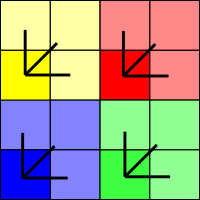
\includegraphics[width=250px]{nearest.pdf}}
        \caption{\label{fig:rungeg} Obrazowanie działania metody najbliższego sąsiada}
    \end{figure}
    \begin{figure}[h]
        \center{\includegraphics[width=330px]{none.png}}
        \caption{\label{fig:rungeg} Powiększenie metody najbliższego sąsiada}
    \end{figure}
    
    \pagebreak

    \subsection{Interpolacja liniowa}
    Wartość piksela jest wyliczana z funkcji interpolującej dwa sąsiednie piksele
    \begin{figure}[h]
        \center{\includegraphics[width=330px]{linear.png}}
        \caption{\label{fig:rungeg} Powiększenie metody interpolacji liniowej}
    \end{figure}

    \pagebreak

    \subsection{Interpolacja kubiczna}
    Działa analogicznie jak liniowa, tylko że wykorzystuje funkcje sześcienne. Obraz otrzymany tą metodą jest bardziej rozmazany lecz wydaje się być bardziej naturalny.
    \begin{figure}[h]
        \center{\includegraphics[width=330px]{cubic.png}}
        \caption{\label{fig:rungeg} Powiększenie metody interpolacji kubicznej}
    \end{figure}
\end{document}